\documentclass[a4paper,titlepage]{article}
\usepackage{ascmac}
\usepackage{amsmath,amssymb}
\usepackage{siunitx}
\sisetup{group-separator = {,}}
\usepackage[dvipdfmx]{graphicx}

\usepackage{listings}
\usepackage{color}

\lstset{
language={Ruby},
basicstyle={\small\ttfamily},
identifierstyle={\small},
commentstyle={\small\ttfamily \color[rgb]{0,0.5,0}},
keywordstyle={\small\ttfamily\bfseries \color[rgb]{1,0,0}},
ndkeywordstyle={\small},
stringstyle={\small\ttfamily \color[rgb]{0,0,1}},
frame={tb},
breaklines=true,
columns=[l]{fullflexible},
numbers=left,
xrightmargin=0zw,
xleftmargin=3zw,
numberstyle={\scriptsize},
stepnumber=1,
numbersep=1zw,
morecomment=[l]{//}
}

\begin{document}
  \title{Process System Engineering \#3}
  \author{\#03150796 Amane Suzuki}
  \date{October 20, 2015}
  \maketitle

  \section{Abstract}
  The purpose of this problem set is to estimate power consumption considering
  that stirring energy go into reactors and produce the heat.

  \section{Algorithm}
  There is a major change in \verb/reactor()/ function. The main structure is,
  \begin{screen}
    \begin{verbatim}
def reactor(gamma_in, gamma_out, prev_energy)
  calc_heat_transfer_rate   #=> h
  calc_dimensionless_number #=> Re, Pr, Nu
  calc_power_consumption    #=> new_energy

  if (new_energy - prev_energy).abs < accuracy
    return results
  else
    return reactor(gamma_in, gamma_out, new_energy)
  end
end\end{verbatim}
  \end{screen}

  In \verb/reactor()/ function, we use Newton's method (Figure.\ref{fig:newton}).

  Given that stirring energy does not go into reactor, we can calculate
  power consumption of each reactor (based on the method which is stated in previous report).

  Power consumption, however, actually go into reactor and produce the heat.

  Therefore, while accuracy is inadequate, \verb/reactor()/ pass power consumption to \verb/reactor()/ repeatedly and modify it.

  \begin{figure}[htbp]
    \centering
    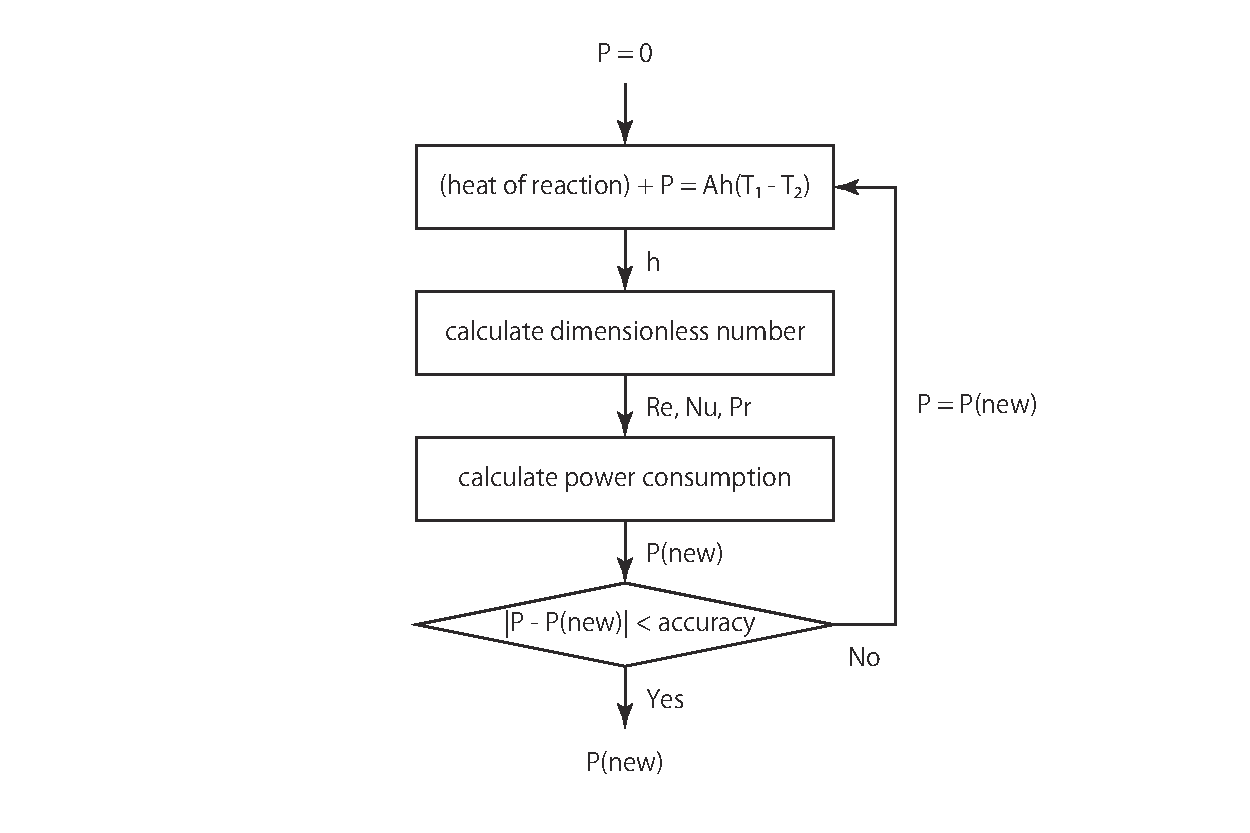
\includegraphics[height=7.2cm]{images/newton.pdf}
    \caption{Routine in reactor() function}
    \label{fig:newton}
  \end{figure}

\newpage

  \section{Result}

  \subsection*{(1)$N=1, \gamma_0=0.05$}
  Use listing \ref{code:normal},
  \begin{screen}
    \begin{verbatim}
$ ruby plant.rb
input n[-], gamma_0[wt%], T2[K]
1
0.05
258
Conditions:
(N, gamma_0, T2) = (1, 0.05, 258)
Reactor Size:
V = 514.706 [m3]
D = 7.959 [m]
H = 10.346 [m]
Results:
#1
Re = 7299.855
n = 0.334 [rps]
P = 38267.204 [W]
Total:
Ptot = 38267.204 [W]\end{verbatim}
  \end{screen}

  \begin{table}[htbp]
    \centering
    \begin{tabular}{cc}\hline
      volume & $\SI{514.706}{\cubic\meter}$ \\
      diameter & $\SI{7.959}{\meter}$ \\
      height & $\SI{10.346}{\meter}$ \\
      total power consumption & $\SI{38.267}{\kilo\watt}$ \\ \hline
    \end{tabular}
    \caption{Result in $(N, \gamma_0, T_2) = (1, 0.05, 258)$}
  \end{table}

\newpage

  \subsection*{(2)$N=3, \gamma_0=0.04$}
  Use listing \ref{code:normal},
  \begin{screen}
    \begin{verbatim}
$ ruby plant.rb
input n[-], gamma_0[wt%], T2[K]
3
0.04
258
Conditions:
(N, gamma_0, T2) = (3, 0.04, 258)
Reactor Size:
V = 153.215 [m3]
D = 5.314 [m]
H = 6.908 [m]
Results:
#1
Re = 11429.325
n = 0.121 [rps]
P = 213.882 [W]
#2
Re = 3632.928
n = 0.153 [rps]
P = 594.829 [W]
#3
Re = 1636.309
n = 0.136 [rps]
P = 522.565 [W]
Total:
Ptot = 1331.275 [W]\end{verbatim}
  \end{screen}

  \begin{table}[htbp]
    \centering
    \begin{tabular}{cc}\hline
      volume & $\SI{151.215}{\cubic\meter}$ \\
      diameter & $\SI{5.314}{\meter}$ \\
      height & $\SI{6.908}{\meter}$ \\
      total power consumption & $\SI{1.331}{\kilo\watt}$ \\ \hline
    \end{tabular}
    \caption{Result in $(N, \gamma_0, T_2) = (3, 0.04, 258)$}
  \end{table}

  \newpage

  \subsection*{(3)show table}
  \begin{screen}
    \begin{verbatim}
$ ruby plant-advanced.rb
593.502 126.602	54.813	31.533	20.908
2729.104	578.714	250.365	143.986	95.456
7790.098	1628.786	703.4	404.237	267.889
18586.917	3770.145	1622.235	930.917	616.453
41466.439	7879.11	3366.358	1926.365	1273.802\end{verbatim}
  \end{screen}

  \begin{table}[htbp]
    \centering
    \begin{tabular}{l|lllll}\hline
      & \multicolumn{5}{c}{$N$} \\
      $\gamma_0$ & 1 & 2 & 3 & 4 & 5 \\ \hline
      0.01 & 593.502 & 126.602 & 54.813 & 31.533 & 20.908 \\
      0.02 & 2729.104 & 578.714 & 250.365 & 143.986 & 95.456 \\
      0.03 & 7790.098 & 1628.786 & 703.4 & 404.237 & 267.889 \\
      0.04 & 18586.917 & 3770.145 & 1622.235 & 930.917 & 616.453 \\
      0.05 & 41466.439 & 7879.11 & 3366.358 & 1926.365 & 1273.802 \\\hline
      \end{tabular}
    \caption{Power Consumption $P [\si{\kilo\watt}]$ in each condition}
  \end{table}

  \newpage

  \section{Source Program}
  \lstinputlisting[caption=plant.rb, label=code:normal]{code/reactor.rb}
\end{document}
